\section{Method}
Figure~\ref{fig:framework} illustrates the overall architecture of \model.
The framework consists of three key components:
(1)~\textbf{Normalize \& Whiten}, where each text view undergoes per-view normalization to address anisotropy;
(2)~\textbf{Cross Network}, which captures explicit ID$\times$Text interactions via DCN-V2;
and (3)~\textbf{Multi-View Alignment}, which uses InfoNCE loss with cold-start reweighting to align text views with ID embeddings.
We elaborate each component below.

\subsection{Backbone: SASRec with Text Fusion}
Let a user interaction sequence be $s_u = [i_1,\dots,i_n]$
with maximum length $L$. \base encodes $s_u$ into a sequence
representation $\mathbf{h}_u \in \mathbb{R}^d$ via a
Transformer. Each item $i$ has an ID embedding
$\mathbf{e}_i \in \mathbb{R}^d$. We augment items with text
features and fuse them into a \emph{fused item embedding}
$\tilde{\mathbf{e}}_i$ used for scoring.

\subsection{Multi-View Text Representations}
We assume a lightweight \tfidf embedding $\mathbf{t}_i^{(0)} \in \mathbb{R}^{d_t}$
as a base view and $V$ \llm prompt views
$\{\mathbf{t}_i^{(v)} \in \mathbb{R}^{d_l}\}_{v=1}^V$ (e.g.,
identity/function/audience/category views), where $d_t$ and $d_l$ denote the
\tfidf and raw \llm embedding dimensions, respectively.

\paragraph{Per-view whitening.}
Multi-view \llm embeddings suffer from three failure modes:
\textbf{(i) scale mismatch}---different views may have vastly
different magnitude distributions, causing some views to
dominate fusion; \textbf{(ii) view correlation}---prompts
eliciting similar semantics produce correlated features that
redundantly encode the same information; \textbf{(iii)
cross-view redundancy}---without decorrelation, the cross
network learns redundant interactions across views rather than
complementary feature crosses.

To address these issues, we first reduce each \llm view from $d_l$ to $d_v$
dimensions via truncated SVD, then apply ZCA whitening~\cite{kessy2018zca} to each view
independently, which decorrelates multi-view channels and makes
subsequent interactions more learnable.
Given the reduced embedding matrix $\mathbf{X}^{(v)} \in \mathbb{R}^{|I| \times d_v}$
for view $v$ over all items, we compute:
\begin{align}
  \mathbf{X}_c^{(v)} &= \mathbf{X}^{(v)} - \boldsymbol{\mu}^{(v)}, \\
  \boldsymbol{\Sigma}^{(v)} &= \frac{1}{|I|}(\mathbf{X}_c^{(v)})^\top \mathbf{X}_c^{(v)}, \\
  \mathbf{X}_w^{(v)} &= \mathbf{X}_c^{(v)} (\boldsymbol{\Sigma}^{(v)} + \epsilon \mathbf{I})^{-1/2},
\end{align}
where $\boldsymbol{\mu}^{(v)}$ is the mean embedding, $\boldsymbol{\Sigma}^{(v)}$
is the covariance matrix, and $\epsilon$ is a small constant for numerical
stability. The whitening statistics are computed offline on the training set
and fixed during training/inference. Each view uses its own whitening
parameters (per-view whitening), which better preserves view-specific
semantics than shared whitening across views.

\paragraph{SE-style channel gating.}
We use an SE-style channel gating for adaptive feature
recalibration, inspired by the channel-wise attention mechanism
in SENet~\cite{hu2018senet}. While the original SENet applies
squeeze (global pooling) followed by excitation, our
implementation directly applies an MLP-based gating over each
projected embedding, which is more suitable for per-item
representations (no pooling across items). Each whitened view
is projected to the backbone dimension $d$ and refined by:
\begin{align}
  \mathbf{z}_i^{(v)} &= \mathbf{W}_v \mathbf{t}_{w,i}^{(v)} \in \mathbb{R}^d,\\
  \mathbf{r}_i^{(v)} &= \mathbf{z}_i^{(v)} \odot \sigma(\mathrm{MLP}_v(\mathbf{z}_i^{(v)})),
\end{align}
where $\mathbf{W}_v \in \mathbb{R}^{d \times d_v}$ is the projection matrix,
$\mathbf{t}_{w,i}^{(v)} \in \mathbb{R}^{d_v}$ is the whitened embedding for
item $i$ in view $v$, and $\mathrm{MLP}_v: \mathbb{R}^d \to \mathbb{R}^d$ is a two-layer
network with reduction ratio $r$.

\paragraph{Per-view $\ell_2$ normalization.}
After SE-style gating, we apply per-view $\ell_2$ normalization
to each view independently. This normalization serves two purposes:
(i) it ensures each view contributes to the fusion on a comparable
scale, preventing views with larger magnitudes from dominating;
(ii) it stabilizes the subsequent cross network learning by
providing well-conditioned inputs:
\begin{equation}
  \hat{\mathbf{r}}_i^{(v)} = \frac{\mathbf{r}_i^{(v)}}{\lVert \mathbf{r}_i^{(v)} \rVert_2 + \epsilon}.
\end{equation}
Together with whitening, per-view normalization addresses scale mismatch
across views while preserving their distinct semantic content: whitening
decorrelates feature dimensions within each view, while $\ell_2$
normalization ensures comparable contribution magnitudes across views.

\paragraph{View gating and fusion.}
We learn a scalar gate $g_v=\sigma(\theta_v)\in(0,1)$ for each
view and \emph{do not} enforce cross-view normalization (each
view independently contributes $0$--$1$). All views (and
optionally the \tfidf base) are concatenated and projected
back to $\mathbb{R}^d$:
\begin{equation}
  \mathbf{t}_i = \mathbf{P}\Big[\mathbf{t}_i^{(0)};\; g_1\hat{\mathbf{r}}_i^{(1)};\; \dots;\; g_V\hat{\mathbf{r}}_i^{(V)}\Big] \in \mathbb{R}^d,
\end{equation}
where $\mathbf{P} \in \mathbb{R}^{d \times (d_t + Vd)}$ is the fusion projection matrix.

\subsection{Explicit Cross Fusion}
Rather than relying solely on self-attention to capture
high-order interactions between collaborative and textual
signals, we introduce an \emph{explicit cross} module based on
DCN-V2~\cite{wang2021dcnv2}. Self-attention in \base models
sequence-level item--item dependencies, but does not
explicitly model feature-level crosses between ID embeddings
and text embeddings. DCN-V2 cross networks fill this gap by
learning high-order ID$\times$text interactions through
element-wise products gated by learned weight matrices.

Given concatenated features
$\mathbf{x}_i=[\mathbf{e}_i;\alpha_i \mathbf{t}_i] \in \mathbb{R}^{2d}$, where
$\mathbf{e}_i \in \mathbb{R}^d$ is the ID embedding and $\mathbf{t}_i \in \mathbb{R}^d$ is the
fused text representation, a cross layer updates:
\begin{equation}
  \mathbf{x}^{(l+1)} = \mathbf{x}^{(l)} + \mathbf{x}^{(0)} \odot (\mathbf{W}_l\mathbf{x}^{(l)} + \mathbf{b}_l),
\end{equation}
where $\mathbf{W}_l \in \mathbb{R}^{2d \times 2d}$ is a
full-rank weight matrix and $\mathbf{b}_l \in \mathbb{R}^{2d}$ is the bias;
$\odot$ denotes element-wise product. We use the full-rank variant of DCN-V2 (non-mix)
rather than low-rank or mixture-of-experts variants. The
cross output $\mathbf{x}^{(C)} \in \mathbb{R}^{2d}$ is combined with a shallow MLP via a predictor
layer to produce the fused embedding $\tilde{\mathbf{e}}_i \in \mathbb{R}^d$.
The scalar $\alpha_i \in (0,1)$ includes a global text gate and
optional per-item gating, scaled by temperature for stable
fusion.

\subsection{Multi-View Contrastive Alignment}
We align each text view to the ID embedding space using
\InfoNCE~\cite{oord2018cpc}. The alignment objective is:
\textbf{text view $\to$ ID space}; positive pairs are
(item's text view, item's ID embedding); negatives are
in-batch items. This ensures that text representations
carry collaborative signals and can serve as drop-in
replacements for ID embeddings in cold-start scenarios.

For a batch of $B$ items, we define
the cosine similarity matrix
$\mathbf{S} \in \mathbb{R}^{B \times B}$ with entries
$\mathbf{S}_{ij} = \mathrm{cos}(\mathbf{e}_{i},
\hat{\mathbf{r}}_{j}^{(v)})$ between ID embeddings
$\mathbf{e}_i \in \mathbb{R}^d$ and text view embeddings
$\hat{\mathbf{r}}_j^{(v)} \in \mathbb{R}^d$, with temperature $\tau$.
The per-view alignment loss is:
\begin{equation}
  \mathcal{L}_{\text{align}}^{(v)} =
  \frac{1}{B}\sum_{i=1}^{B}
  -\log \frac{\exp(\mathbf{S}_{ii}/\tau)}{\sum_{j=1}^{B}\exp(\mathbf{S}_{ij}/\tau)}.
\end{equation}
We learn view weights $\pi_v=\mathrm{softmax}(\boldsymbol{\phi})_v$
and combine per-view losses:
\begin{equation}
  \mathcal{L}_{\text{mv-align}} = \sum_{v=1}^{V}\pi_v \mathcal{L}_{\text{align,w}}^{(v)}.
\end{equation}

We enhance cold-start item performance through two complementary
mechanisms that operate at different stages:

\paragraph{Training-time cold-start reweighting.}
To avoid alignment being dominated by frequent items, we
reweight samples based on item popularity $\mathrm{pop}(i)$
during training, where $\mathrm{pop}(i)$ is the interaction count:
\begin{equation}
  w_i = 1 + \beta\cdot \max\Big(0, \frac{P_0-\mathrm{pop}(i)}{P_0}\Big),
\end{equation}
where $P_0$ is the cold-start threshold (items with $\mathrm{pop}(i) < P_0$
receive boosted weights). The weighted alignment loss becomes:
\begin{equation}
  \mathcal{L}_{\text{align,w}}^{(v)} =
  \frac{1}{\sum_i w_i}\sum_{i=1}^{B} w_i \cdot
  \left[-\log \frac{\exp(\mathbf{S}_{ii}/\tau)}{\sum_{j=1}^{B}\exp(\mathbf{S}_{ij}/\tau)}\right],
\end{equation}
where $w_i$ only reweights the anchor (positive) samples, ensuring
that cold-start items receive sufficient gradient updates during
alignment training.

\paragraph{Inference-time cold-start boosting.}
To complement training-time reweighting, we apply adaptive text
weighting during inference. For an item $i$ with popularity
$\mathrm{pop}(i)$, we compute a dynamic boost factor:
\begin{equation}
  \gamma_i = 1 + \beta_{\text{infer}} \cdot \max\Big(0, 
  \frac{P_0-\mathrm{pop}(i)}{P_0}\Big),
  \label{eq:infer_boost}
\end{equation}
where $\beta_{\text{infer}}$ is the inference boost coefficient.
The effective text weight in the fusion layer becomes 
$\alpha_i' = \alpha_i \cdot \gamma_i$, dynamically increasing text
reliance for cold-start items without modifying model parameters.
This decoupling allows deployment-time adjustment without
retraining: lower $\beta_{\text{infer}}$ for balanced performance,
or higher $\beta_{\text{infer}}$ for cold-start prioritization
(see Appendix~\ref{app:hyper} for validated configurations).

Together, these two mechanisms ensure that cold-start items receive
both strong learning signals during training (via reweighted
alignment) and appropriate inference-time emphasis (via dynamic
boosting), enabling effective cold-start recommendations without
sacrificing performance on frequent items.

\begin{figure}[t]
\centering
\IfFileExists{figures/framework.pdf}{%
  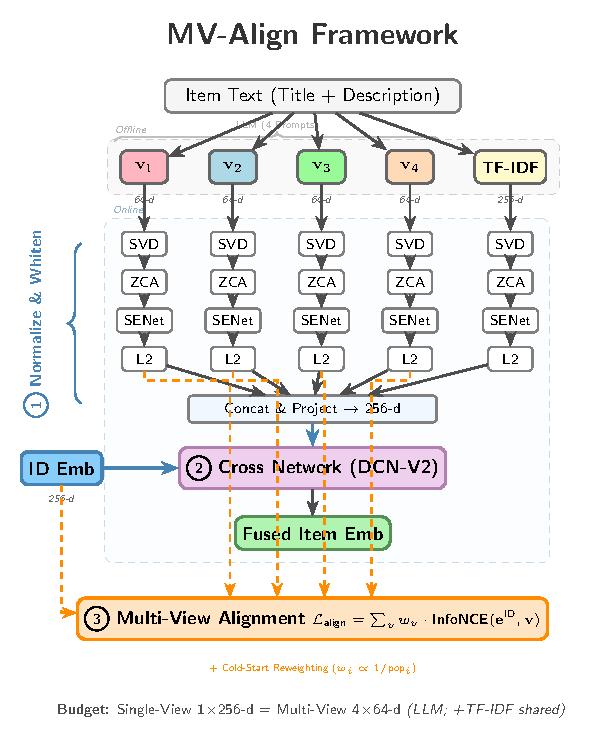
\includegraphics[width=\linewidth]{figures/framework.pdf}%
}{%
  \fbox{\parbox[c][0.22\textheight][c]{0.95\linewidth}{\centering
  \textbf{Framework figure placeholder.}\\
  Put `framework.pdf` under `paper_sigir/figures/`.}}%
}
\caption{Overview of the MV-Align framework. The architecture consists of three key components:
\circled{1}~\textbf{Normalize \& Whiten}: each view (4 LLM prompts + TF-IDF) undergoes SVD, ZCA whitening, SE-style gating, and L2 normalization;
\circled{2}~\textbf{Cross Network}: DCN-V2 captures explicit ID$\times$Text interactions;
\circled{3}~\textbf{Multi-View Alignment}: InfoNCE loss with cold-start reweighting aligns each view to ID embeddings.
Embedding budget: single-view uses 1$\times$256-d while multi-view uses 4$\times$64-d (LLM only; TF-IDF 256-d shared).}
\label{fig:framework}
\end{figure}

\subsection{Training Objective}
We optimize:
\begin{equation}
  \mathcal{L} = \mathcal{L}_{\text{rec}} + \lambda \cdot \mathcal{L}_{\text{mv-align}},
\end{equation}
where $\mathcal{L}_{\text{rec}}$ is the standard sequential
recommendation loss (cross-entropy over sampled
positives/negatives in training), and $\lambda$ is the
alignment weight.

\subsection{Model Complexity}
We analyze the space (parameter) and time complexity of each
model variant, following the analysis in~\cite{kang2018sasrec}.
Let $|I|$ denote the number of items, $L$ the maximum sequence
length, $d$ the hidden size, $B$ the batch size, $d_t$ the
\tfidf feature dimension, $d_l$ the \llm embedding dimension,
$V$ the number of text views, and $d_v$ the per-view \llm
dimension.

\paragraph{Space complexity (parameters).}
Table~\ref{tab:complexity} summarizes the parameter and time complexity for each configuration:

\begin{table*}[t]
\caption{Parameter and time complexity of model variants.
$|I|$: \#items, $L$: sequence length, $d$: hidden size,
$d_t$: \tfidf dim, $d_l$: \llm dim, $V$: \#views, $d_v$: per-view dim.}
\label{tab:complexity}
\centering
\small
\begin{tabular}{lll}
\toprule
\textbf{Model} & \textbf{Space Complexity (Parameters)} & \textbf{Time Complexity (per batch)} \\
\midrule
\base (ID-only) & $O(|I|d + Ld + d^2)$ & $O(L^2d + Ld^2 + |I|d)$ \\
\base + \tfidf & $O(|I|d + Ld + d^2 + d_t d)$ & $O(L^2d + Ld^2 + |I|d_t d + |I|d)$ \\
\base + \tfidf + \llm (single-view) & $O(|I|d + Ld + d^2 + (d_t{+}d_l)d)$ & $O(L^2d + Ld^2 + |I|(d_t{+}d_l)d + |I|d)$ \\
\model (multi-view) & $O(|I|d + Ld + d^2 + Vd_v d + d_t d)$ & $O(L^2d + Ld^2 + V|I|d_v d + |I|d)$ \\
\bottomrule
\end{tabular}
\end{table*}

\paragraph{Space breakdown.}
The \base backbone contributes $O(|I|d)$ for item embeddings,
$O(Ld)$ for position embeddings, and $O(d^2)$ for the
Transformer encoder parameters (self-attention $Q,K,V,O$
projections and point-wise FFN layers; the number of layers
is a small constant). Text variants add projection layers
proportional to the text feature dimension: \tfidf adds
$O(d_t d)$, single-view \llm adds $O((d_t + d_l)d)$, and
multi-view adds $O(V d_v d)$ for per-view projections and
SE-style gating modules plus $O(d_t d)$ for the base view. Cross layers
contribute $O(d^2)$ each (we use a single cross layer),
absorbed into the backbone $O(d^2)$ term.

\paragraph{Time breakdown.}
The Transformer self-attention layer costs $O(L^2d)$ for
computing the $L\times L$ attention matrix, plus $O(Ld^2)$
for the point-wise FFN. Full-ranking scoring adds $O(|I|d)$
for computing logits over all items. Text models incur
additional fusion overhead:
\begin{itemize}[leftmargin=*,itemsep=1pt]
  \item \textbf{\tfidf}: Text projection $O(|I| d_t d)$ for all items.
    Cross network fusion is $O(|I| d^2)$, absorbed since $d_t \approx d$.
  \item \textbf{Single-view}: Projection cost increases to
    $O(|I| (d_t + d_l) d)$ due to larger input dimension.
  \item \textbf{Multi-view}: Per-view projection $O(V |I| d_v d)$;
    concat and cross costs are absorbed since $V d_v \approx d_t \approx d$.
\end{itemize}
Alignment loss adds $O(B^2 d)$ per view for InfoNCE similarity
matrix computation. Note that \llm embeddings are
\emph{precomputed offline} and stored as static buffers; the
online inference cost is dominated by projection layers
rather than the \llm encoder.
